\newif\ifdraft
\ifx\dontdraft\relax
\message{IFX TRUE}
\draftfalse
\else
\message{IFX FALSE}
\drafttrue
\fi

\draftfalse

\def\fig#1{Fig.~\ref{#1}}

% Final version: use times!
% \documentstyle[times,graphicx,ht01e]{article}
\documentclass[twocolumn]{IV02}
\usepackage[latin1]{inputenc}
\usepackage{graphicx}
\usepackage{times}
\ifdraft
\usepackage{beton}
\fi
% \draftfalse

\ifdraft
\renewcommand{\baselinestretch}{0.9}
\def\margincomment#1{
\marginpar{
\vbox{
\scriptsize #1
}
}}
\def\nakki#1{\marginpar{\bf Nakki: #1}}
\pagestyle{plain}
\else
\def\margincomment#1{}
\def\nakki#1{}

% % Make the times fonts defaults again if not draft.
%  \renewcommand{\sfdefault}{phv}
%  \renewcommand{\rmdefault}{ptm}
%  \renewcommand{\ttdefault}{pcr}

\fi


% Define a macro for your own margin notes here
% If it is ABSOLUTELY clear that something is a typo, go ahead
% and fix it. But don't make any major changes to the text itself
% yet. Also, only propose rearrangements in the margin: CVS doesn't
% work too well with rearrangements and edits done by several
% people. I will be the editor until wed or thu.
\def\tjl#1{\margincomment{Tjl: #1}}
\def\vp#1{\margincomment{vp: #1}}
\def\rr#1{\margincomment{rr: #1}}
\def\cat#1{\margincomment{cat: #1}}
\def\ajk#1{\margincomment{ajk: #1}}
\def\jvk#1{\margincomment{jvk: #1}}
\def\benja#1{\margincomment{benja: #1}}
\def\marke#1{\margincomment{marke: #1}}


% \documentstyle[times,graphicx,uist,isolatin1]{article}
\begin{document}

\newcommand{\url}[1]{{\fontsize{9pt}{8pt}\fontfamily{phv}\fontseries{c}\selectfont{#1}}}
\newcommand{\hyp}{\discretionary{}{}{}}


\bibliographystyle{plain}
\title{
Fillets:
Cues for Connections 
in Focus+Context Views
of Graph-like Diagrams 
}

\author{
\vbox{
\hbox{
\hbox{\parbox[t]{8.9cm}{\centering
 {Tuomas J. Lukka\ \ \ and\ \ \ Janne V. Kujala}\\
  Hyperstructure Group\\
  Dept.~of Mathematical Information Technology\\
  University of Jyv\"askyl\"a, PO.~Box~35\\
  FIN-40351~Jyv\"askyl\"a\\
  Finland\\
  {\tt lukka@iki.fi}}}~\hbox{\parbox[t]{8.9cm}{\centering
 {Marketta Niemel�  }\\
  Dept.~of Computer Science and Information Systems\\
  University of Jyv\"askyl\"a, PO.~Box~35\\
  FIN-40351~Jyv\"askyl\"a\\
  Finland\\
  }}
}
}
}

\maketitle

\ifdraft
\textwidth 6.6cm
\columnwidth 8.6cm
\onecolumn
% \textwidth 8.5cm
\marginparwidth 8.5cm
\fi

% \textwidth 3.5in
% \columnwidth 3.5in

\begin{abstract}
We apply fillets --- smoothing of sharp angles at the joints ---
between the connections and nodes of graph-like diagrams.

In situations where the graph layout is constrained,
e.g.~Focus+Context views or views where the coordinates of the nodes
are informative, fillets can clarify the relationships considerably without
altering the layout.

A visual search experiment supports our hypothesis
that with fillets it is considerably easier to perceive 
node-connection structures.

% However, they do not seem
% to be preattentively found.

% 
% Edgeless connections, i.e.~thick connections which smoothly blend to
% nodes at both ends so that there are no node edges between the two
% cells help see the connections.
% 
% In visualizations, the 
% horizontal/vertical/diagonal direction of the edges is significant.
% Also, there is usually significant content in each node, from a few words
% to a paragraph of text.
% \benja{Isn't the horizontal/vertical/diagonal especially important in ZZ,
%        though of some admitted use elsewhere? If so, it would be worth
%        saying that this is especially a problem in the area we are
%        researching visualizations for.}
% \tjl{ This was about zz. Don't know why it was still here. }

We discuss algorithms with different tradeoffs for flexibility and performance
for rendering these connections 
in a single pass using
OpenGL.
\end{abstract}


% \tolerance=400 
\tolerance=500 
  % makes some lines with lots of white space, but      
  % tends to prevent words from sticking out in the margin

\def\vob{{\tt Vob}}
\def\vobscene{{\tt VobScene}}
\def\view{{\tt View}}
\def\key{{\tt key}}
\def\diff{{\tt diff}}

\def\unfin{\tiny}
\def\fin{\normalsize}


\section{Introduction}

Graph-like diagrams are usually drawn using 
nodes (generally boxes or circles)
and lines between them for connections\cite{herman00graph}.
% For examples, see UML (ref) and (ref infvis).
% \benja{And mind-map like labeling of the arcs, see e.g. IsaViz at
%        http://w3.org/2001/11/IsaViz/.}
If the graph is simple (e.g.~a tree), or
the layout is good, the way of drawing the nodes and edges
does not matter much.

However, sometimes
connections must
cross other connections or nodes frequently.
This happens, for example,
in Focus+Context\cite{fc-taxonomy} views of multiply connected (non-planar)
graphs, or
when the connections have to leave the nodes in specified directions,
or when there are
other constraints to the layout.
The Vanishing View of Gzz\cite{gzz} to the ZigZag structure\cite{zigzag-manual}
is one example: here, the layout of the nodes (cells) and the directions
the connectors leave the cells are determined by the underlying structure:
a horizontal connector is different from a vertical one.


% 
% \begin{figure}
% \fbox{\vbox{\hbox to 7cm{A} \vskip 2in}}
% \caption{
% \label{fig-zzspace}
% A nontrivial ZZ space shown using nodes and lines.
% A screenshot of Gzz.
% }
% \end{figure}
% 
% 
% This stems from the way people draw diagrams on
% paper: first the nodes are drawn and only then the 
% connection between them. When a node is being drawn, 
% connections it are not anticipated and therefore they cannot
% cause any changes in the outline of the node.\footnote{
% Naturally, given time, a human can produce any kind of illustration;
% here we are discussing the case of drawing simple diagrams as a part
% of a thought process, not illustrating a book}.
% 


% 
% 
% Computers we do not have the same limitations:
% all connections to a node are known at the outset; if some connection
% changes, the whole diagram can be redrawn.
% Also, unlike for humans, there is no significant effort in
% erasing parts of what was already drawn.
% 
% Currently most computer-drawn 2D diagrams mimic the human hand-drawn diagrams,
% even though the tradeoffs involved are quite different.
% \benja{This sounds too much like how Ted would structure an argument:
%        ``It simulates paper, so it's bad. For example...'' Instead, first
%        say why it's bad, then say `and that is because it emulates paper'.}


In such situations,
the pure node-line diagrams are 
inherently
ambiguous, as shown in Fig.~\ref{fig-boxline-ambiguity} a).
In order to be able to understand such diagrams
if the layout cannot be changed (or if that would lead to other complications), 
a rendering method which allows the viewer to distinguish between the 
different possibilities is needed.


% In a diagram that has been designed by a human, the resolution of
% the ambiguity is obvious: a human would simply never draw the diagram 
% in 
% Fig.~\ref{fig-boxline-ambiguity}a)
% to mean Fig.~\ref{fig-boxline-ambiguity}c).

\begin{figure}
%\fbox{\vbox{\vskip 2in}}
\centering
\includegraphics[width=6cm]{boxline-ambiguity.eps}
\caption{
\label{fig-boxline-ambiguity}
An extreme example of
the visual ambiguity inherent in complex boxes-and-lines diagrams
when the layout is restricted:
a) the ambiguous diagram, b), c) possible meanings. If the diagram
was designed by a human, one can be certain that b) is the correct 
interpretation.
}
\end{figure}

% 
% Computers are often draw diagrams 
% several orders of magnitude more complex than humans. 
% In the human-drawn diagrams the connection lines almost never go behind
% an object, but in the more complex diagrams that computers need to draw,
% achieving this is not necessarily possible or desirable. 
% In order to be visually
% clear, the nodes need to be laid out in a reasonable manner and the 
% connections must go in relatively straight lines.
% 
% 
% \benja{Suggested structure for introduction:
%        \begin{enumerate}
%        \item The problem: why attentive processing is bad
%        \item Research on pre-attentive processing
%        \item A structure in need for that: complex graphs
%        \item Good 2D layout of graphs is difficult
%        \item Geons: have the same problem
%        \item Good for planar and F+C graph views; not very useful for trees
%        \item Problem is: conns go under nodes
%        \item When humans draw them, those aren't ambiguous; but the diagrams
%              humans draw are much smaller, too
%        \item Refer to different figures, ink-draw ereasing technique and so on
%        \item (but these aren't pre-attentive)
%        \item In this article, we show an alternative approach that makes
%              use of pre-attentive processing...
%        \end{enumerate}
% }
% 
%
%In interactive focus+context visualizations of large data sets
%it is usually not possible to maintain a 2D layout
%without overlapping nodes and connections.

% In this article, 

% NON-TREE

% NON-PLANAR
% \benja{Give examples of what one would want to use that for. -- I think
       % that actually real non-planar graphs aren't that important; the
       % point is that if you have a dense graph of many interconnected nodes,
       % showing them in a planar view is quickly incomprehensible, and
       % focus+context can help. But when you're using focus+context, you
       % cannot have the user optimize it so that no connections go under
       % nodes, and thus you can gain a lot from fillets.}

One possibility is a technique used in conventional ink
drawing techniques where the lines that go behind an object
do not actually touch the object, as in 
Fig.~\ref{fig-ink-erase}.
% This approach has been used in non-photorealistic rendering (refs) and
% is fairly easy to implement on computers.

\begin{figure}
%\fbox{\vbox{\vskip 2in}}
\centering
\includegraphics[width=6cm]{ink-erase.eps}
\caption{
\label{fig-ink-erase}
An approach in traditional drawing for showing one element going behind 
another by erasing the line.  
}
\end{figure}

Even though this approach helps, it only allows
a human to distinguish between the situations in
Fig.~\ref{fig-boxline-ambiguity}b)
and Fig.~\ref{fig-boxline-ambiguity}c)
by actually directing his/her focus of
attention to the crossing. An explanation can
be found in Fig.~5.5 on p.166 of \cite{ware-info-vis}:
pre-attentive processing cannot distinguish between
juncture/non-juncture. The other examples of pre-attentive/non-pre-attentive
features in the same
book clearly demonstrate that having a pre-attentive 
cue for the connection/nonconnection could
significantly help the viewer to perceive
the structure.

In this article, we explore fillets, a novel approach 
to resolving the ambiguity.
The following sections describe fillets and discuss an experiment 
demonstrating the advantage of fillets in simple graphs.
The implementation of fillets using OpenGL is discussed in the Appendix.


% 
% \section{Motivation: Non-planar Focus+Context Views}
% 
% 
% 
% The intended use of Gzz is very different from the uses of 
% usual graph visualization software.
% 
% Much work has been done on visualizing trees\cite{XXX}. 

% Vanishing
% Focus+context
% depth
% fog
% animation

% Usually\cite{herman00graph} graph visualization has concentrated
% on graphs where the edges are typeless, i.e. either they have no labels
% or (almost) all have separate labels.
% 
% In this work, we are mostly


\section{Fillets}

{\em Filleting}, or rounding corners of surfaces, is 
used in mechanical engineering to improve 
the properties of cast objects.
Sharp corners are fragile and can also cause
defects during molding.
Filleting is an instance of a more general technique
known as {\em blending} - creating surfaces that 
meet several existing surfaces smoothly\cite{rockwood-blending-implicit}.



Figure \ref{fig-fillets} shows how fillets can be used
to avoid the ambiguity in Fig.~\ref{fig-boxline-ambiguity}.
The connection which goes under the middle node seems to do 
so almost three-dimensionally.
% A more complicated view where the advantage of fillets 
% becomes clearer is shown in \fig{fig-zzspace-fillets}.

\begin{figure}
%\fbox{\vbox{\vskip 2in}}
\centering
\includegraphics[width=6cm]{edgeless.eps}
\caption{
\label{fig-fillets}
Fillets resolve the ambiguity of Fig.~\ref{fig-boxline-ambiguity} clearly.
}
\end{figure}

There are two interacting graphical elements in 
fillets. First, the connection is blended smoothly
onto the node, without a derivative discontinuity.
Second, there is no black edge on the connection between the two
nodes (unless there is something on top of the connection).
Together, these two features make it easy to distinguish
between the cases where a connection enters a node or goes under it.

A filleted connection conforms to the Gestalt principle of good continuation. Smoothly changing contours enable more efficient perceptual grouping of visual elements \cite{humphreysviscogn}, in this case, grouping of the node and the connection.  

This use of fillets is entertainingly analogous to the use in mechanical
engineering: fillets ensure that the human perception system
doesn't break an object and a connection starting
from it into two distinct objects.

One might object that fillets might take more space than standard box-line
diagrams.
However, the actual space increase is marginal and is compensated by
the clarity of the view: nodes can overlap more freely without
making it difficult to understand the diagram.

Also, it might be said that
the blending makes the background more solid and so the cells
and connections might be perceived as the outside of the figure
(figure-ground ambiguity).
However, cues such as color, text on the nodes, animation, shading, and fog 
can be used to prevent this.

% 
% The diagram with filleted
% connections can be perceived in two different ways:
% as a single object with a complicated shape or, like the "boxes and
% lines" diagram, as connected pieces. The human eye can choose whichever
% representation is more convenient for the task at hand.
% 
% 
% There are many ways to make connectedness
% pre-attentively differentiable. Making the point of connection
% different from the point of overlap in almost any graphical way
% is sufficient; example, color, thickening of the connecting line, or 
% an arrow end would all work fine.
% 
% \begin{figure}
% \fbox{\vbox{\hbox to 7cm{A} \vskip 2in}}
% \caption{
% \label{fig-zzspace-fillets}
% A nontrivial ZZ space shown using
% filleted
% connections. Contrast with Fig.~\ref{fig-zzspace}.
% A screenshot of Gzz.
% }
% \end{figure}

% 
% We can offer anecdotal evidence that these figures are quite difficult
% to draw by hand; to create the hand-drawn Fig.X the author first had to
% draw a sketch and then draw the final figure very carefully; the reflexes
% for closing the box edge are very strong.
% 

\section{Experiment}

A filleted
connection consists of two visual features, 
widening and borderlessness of the connection. This experiment 
was designed to explore the effect of widening, borderlessness, 
and gaps (as in Fig.~\ref{fig-ink-erase}) 
of the connections on search efficiency
in node-link graphs. The paradigm of visual search, in which the target search 
time is measured as a function of the number of distractor elements, 
was applied (e.g., \cite{treismangelade,treismangormican,wolfe94guided}).
Our main hypothesis was that visual segregation between connections 
entering a node or going behind a node is more effortless
with filleted connections than 
connections without widening, borderlessness (i.e., with borders), or both.
Gaps should facilitate search when filleted 
connections are not implemented. 
In addition, the effect of the visual width of connections as itself (without fillets) was tested. We expected that the width of the connection would not make a difference on search time.
 
\subsection{Method}

\emph{Participants.} Ten participants, seven females and three males, 
perfomed the experiment for a small monetary reward. Their ages 
ranged from 19 to 40 years. All of them participated in all conditions.

\emph{Design and materials.} In the experiment, there were seven
conditions with different combinations of the three main features. 
One variation (no widening, no borderlessness, and no gap) 
was not implemented since there would be no way to distinguish 
between a connection entering a node or going behind a node.
Instead of this, one condition with narrow line-type connection 
was implemented. The eight conditions are listed in Table~\ref{tab-conditions}
and
Fig.~\ref{fig-conditions}. 
Gap width was 1.2 times the width of node border.

\begin{table}
\centering
\begin{tabular}{c|llll}
	Condition & Widening & Borderlessness & Gap & Thick \\
	\hline
	\textbf{1} & \textbf{yes} & \textbf{yes} & \textbf{yes} & \textbf{yes} \\
	2 & no  & yes & yes & yes \\
	3 & yes & no  & yes & yes \\
	4 & no  & no  & yes & yes \\
	5 & no  & no  & yes & no  \\
	\textbf{6} & \textbf{yes} & \textbf{yes} & \textbf{no} & \textbf{yes} \\
	7 & no  & yes & no  & yes \\
	8 & yes & no  & no  & yes 
\end{tabular}
\caption{\label{tab-conditions}
Visual features in the eight conditions. 
Conditions with filleted connections are indicated in bold text}
\end{table}

\def\condscale{.27}

\begin{figure}
\centering
%\begin{tabular*}{7cm}{cc}
1)
\includegraphics[scale=\condscale]{cond0.eps}%
5)
\includegraphics[scale=\condscale]{cond4.eps}\\
2)
\includegraphics[scale=\condscale]{cond1.eps}%
6)
\includegraphics[scale=\condscale]{cond5.eps}\\
3)
\includegraphics[scale=\condscale]{cond2.eps}%
7)
\includegraphics[scale=\condscale]{cond6.eps}\\
4)
\includegraphics[scale=\condscale]{cond3.eps}%
8)
\includegraphics[scale=\condscale]{cond7.eps}\\
%\end{tabular*}
\caption{\label{fig-conditions}
Simple examples of the eight conditions showing a situation
in which a connection goes behind a node.
}
\end{figure}

\begin{figure}
\centering
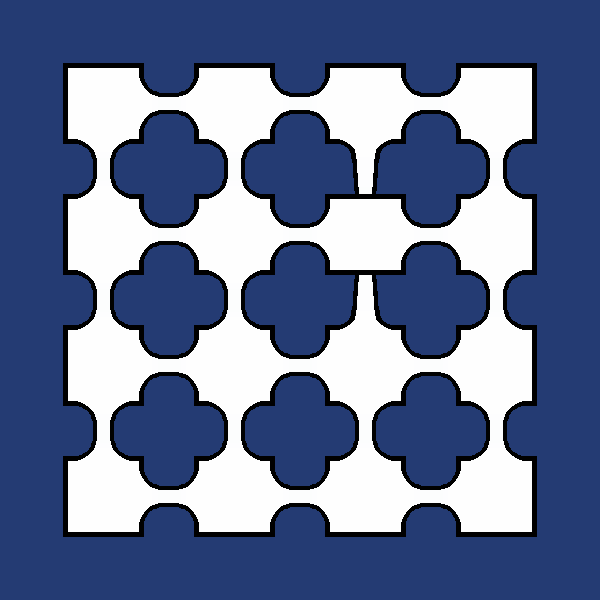
\includegraphics[width=6cm]{grid4x4.eps} \\
\caption{\label{fig-grid}
Condition 1 with 4x4 grid size.
}
\end{figure}



On the test figures, 
nodes were in a regular grid in which all nodes except 
nodes on the edges and the target node were connected 
to four neighbouring 
nodes. At the target node, a connection went behind the node 
either in vertical or horizontal direction (Fig.~\ref{fig-grid}). 
Grids of sizes 4x4, 6x6, or 8x8 were tested to find 
out whether the search time was independent of the set-size, 
which would indicate that the target node was perceived preattentively. 
Node size was equal across all conditions and grid sizes.


\emph{Procedure.} The participants were tested individually. They 
performed all conditions in a random order. One condition consisted 
of 24 trials, among which the three different grid sizes were 
presented randomly, eight trials of each size. A trial started with a fixation point appearing on the computer display for 1.5 sec. Then
a node grid was shown and it remained on until the participant responded. 
The location of the target in the grid was randomized 
(target was never a corner node). 
The task of the participants was to find the target node and 
to choose whether the target was on the left or on the right side 
of the grid. The participant would indicate this by pressing 
either the left or right control key in the keyboard. The participants 
were requested to do this task as fast as possible. The feedback 
was a plus or minus sign on the display, which was shown for 1 sec, thus the pause between two 
successive trials was 2.5 seconds. Each condition began with a practice block of three trials, one of each size. The participant was allowed to perform the practice block twice if desired.
Search time and correctness 
were collected for each test trial.

\subsection{Results}
The search times and errors (Tab.~\ref{tab-ERandER}) were analysed with the repeated measures 
analysis of variance.

% 
% \begin{figure}
% \centering
% 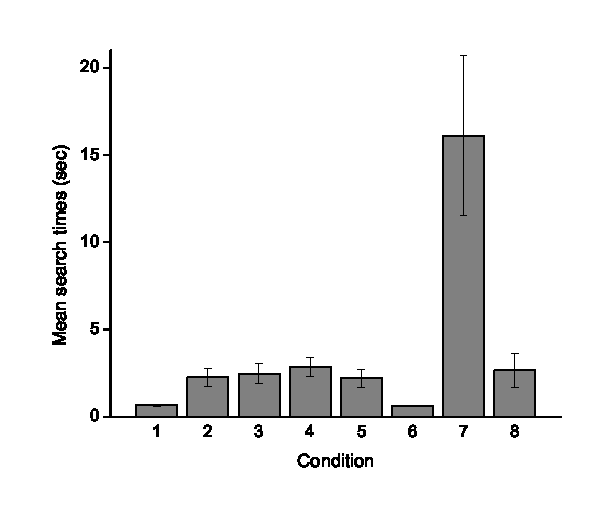
\includegraphics[width=7cm]{RTbycond.eps}
% \caption{
% \label{fig-RTbycond}
% }
% \end{figure}

\begin{figure}
\centering
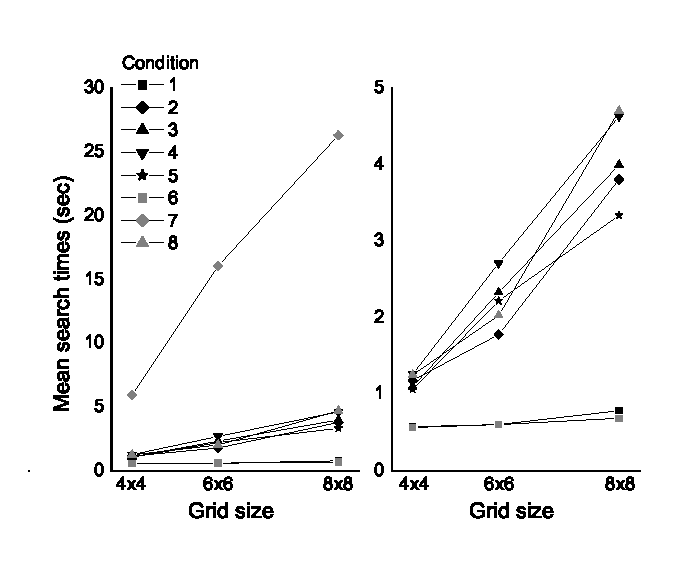
\includegraphics[width=7cm]{RTsbysize2.eps}
\caption{
\label{fig-RTsbysize}
Mean search times in conditions as a function of grid size. 
The two flat lines are conditions 1 and 6 (both filleted), 
the steepest slope is in condition 7. 
The right side is a scaled version of the left side (condition 7 is 
not visible).
}
\end{figure}

\begin{table}
\centering
\begin{tabular}{c|rrr|r}
             &  \multicolumn{3}{c|}{GRID SIZE} & \\
CONDITION    &  16   &  36   &  64   &  Mean \\
\hline
1            &  577  &  608  &  786  &  657 \\
             &  0.00 &  0.00 &  0.00 &  0.00 \\
\hline
2            &  1181 &  1782 &  3809 &  2257 \\
             &  0.00 &  0.00 &  0.00 &  0.00 \\
\hline
3            &  1100 &  2332 &  4000 &  2477 \\
             &  1.25 &  1.25 &  2.50 &  1.67 \\
\hline
4            &  1265 &  2714 &  4634 &  2871 \\
             &  0.00 &  1.25 &  0.00 &  0.42 \\
\hline
5            &  1067 &  2223 &  3339 &  2210 \\
             &  1.25 &  1.25 &  1.25 &  1.25 \\
\hline
6            &  568  &  608  &  687  &  621 \\
             &  0.00 &  0.00 &  0.00 &  0.00 \\
\hline
7            &  5964 &  16064&  26326&  16118 \\
             &  6.25 &  0.00 &  3.75 &  3.33 \\
\hline
8            &  1254 &  2032 &  4705 &  2663 \\
             &  0.00 &  1.25 &  0.00 &  0.42 \\
\hline
Mean         &  1622 &  3545 &  6036 &  3734 \\
             &  1.09 &  0.63 &  0.94 &  0.89 
\end{tabular}
\caption{
\label{tab-ERandER}
Correct search times (msec) and error rates (\%) by condition and grid size
}
\end{table}

\begin{table}
\centering
\begin{tabular}{c@{\hspace{3pt}}ccrl}
\hline
\multicolumn{2}{c}{Compared} & Fixed &  & Statistical \\
\multicolumn{2}{c}{conditions} & features & $F(1,9)$ & significance \\
\hline
no W & W \\
\hline
2 & 1 & B,G & $58.5$, & $p < .001$ \\
4 & 3 & G   & $2.9$,  & $p > .05$ \\
7 & 6 & B   & $57.0$, & $p < .001$ \\
\hline
no B & B \\
\hline
3 & 1 & G,W & $60.4$, & $p < .001$ \\
4 & 2 & G   & $18.2$, & $p < .01$ \\
8 & 6 & W   & $27.0$, & $p < .01$ \\
\hline
no G & G \\
\hline
6 & 1 & B,W & $1.1$, & $p > .05$ \\
7 & 2 & B   & $46.5$, & $p < .001$ \\
8 & 3 & W   & $0.2$, & $p > .05$ \\
\hline
narrow & thick \\
\hline
5 & 4 & G   & $4.2$, & $p > .05$ \\
\hline
\end{tabular}
\caption{
\label{tab-anova-pairwase}
ANOVA table of pairwise comparisons of the conditions. 
The fixed features column shows which other features
were implemented in the compared conditions (W - widening, B - borderlessness, G - gap).
}
\end{table}

\emph{Search times.} The mean correct search times in the eight conditions 
differed from each other [$F(1.1, 10.2) = 48.0$, $p <.001$]. 
The search times were clearly fastest in conditions 1 and 6, 
in which connections were filleted (i.e.~both widening and borderlessness)
[$F(1,9) = 93.4$, $p <.001$]. 
Excluding the obviously different condition 7 did not change this.

The effects of the four visual features - widening, borderlessness, gap, and 
connection width - were analysed by comparing 
the conditions in a pairwise fashion. The results of the analyses are 
collected in Table \ref{tab-anova-pairwase}. 
Widening 
facilitated search only when combined with borderlessness. 
Borderlessness was helpful in any condition, except when connection 
gap was not implemented (again condition 7; see discussion below). 
Gaps did not affect search time when used with widening, either with 
or without borderlessness. Width of the connection 
did not make a difference on search time.

Grid size had a main effect on search time [$F(2,18) = 33.5$, 
$p <.001$], and there was interaction between condition and 
grid size [$F(1.5, 13.4) = 11.8$, $p <.01$]. Search times as 
a function of grid size are shown in Fig.~\ref{fig-RTsbysize}. 
Search times were linearly dependent on grid size also in conditions 
1 and 6 [$F(2,18) > 11.2$, $p <.001$ for both conditions]. 
Thus it seems that although graphs with fillets 
are undoubtedly most efficient to search, a connection going behind 
a node is not found during preattentive visual processing but 
requires attentive search.

\emph{Errors.} Error rates depend on condition [$F(2.5, 
22) = 4.2$, $p <.01$] but not grid size [$F(2, 18) =.6$, $p >.05$]. 
There is no interaction effect between condition and grid size 
[$F(4.5, 40.4) = 1.8$, $p >.05$]. Condition
7 was most error-prone (3.3\%). 

To summarize, the results of the experiment support our hypothesis that 
in a node-link graph with filleted connections,
it is easier to distinguish between connections going either 
behind a node or into a node. Search in fillet graphs was quite 
unsensitive to the addition of non-target nodes, even close to 
parallel (preattentively processed) when compared to searches 
in the other graphs in the experiment. 


We expected a gap between a connection and a node to facilitate search when 
fillets were not implemented but it did not. 
Probably the gap width used in the experiment was too small to be  
effortlessly found. The width of the connection had no effect 
on search efficiency, as expected. 


In condition 7, search times and error rates
were especially long when compared 
to the other conditions. 
One possible explanation is that
a Hermann Grid illusion\cite{spillmanhermanngrid}
is created
in the junction of a connection and a node.
This means that 
if not directly in the focus of the eye,
the junction area appears darker than the node or the connection, 
which makes it hard to distinguish between a target and non-target junctions. 

\section{Conclusion}

There has been much research on graph visualization recently.
However, the research seems to have been mostly concentrated on 
graph and tree layout and Focus + Context methods.

The one significant exception we have found in 
the literature is the work of Irani, Tingley and Ware
on
geon diagrams\cite{irani-diagrams,irani01using}.
Geon diagrams
use basic 3D geometric shapes as building blocks\cite{biederman87} for
diagrams, 
aiming at making the parts of the diagram more easily
recognizable.

However, the geon diagrams do not necessarily help much in the 
ambiguity of Fig.~\ref{fig-boxline-ambiguity}; their point is 
in making the {\em types} of connections recognizable, not in helping
to understand the {\em connectivity} itself.

In this article, we have introduced fillets as a way of improving
perception of node-line structures.
With filleted connections, it is easier to discriminate whether a connection
enters a node or goes behind it. 
Fillets are useful in constrained layouts where the number of crossing
edges cannot be minimized for some reason.

% COMMENT: If the goodness of fillets is based on node shape (see below), 
% the width of the connection should not matter. Width did not matter in the 
% conditions without fillets. --> Filleted connections should be good also
% with narrow line connections.
% 
% (square cells were used in the experiment, while the usual zz views
% use vertically much thinner cells XXX ???)

% 
% Although geons are 3D structures, a good 2D layout
% is still important in identifying the joints between
% geons. 
% This limits the complexity of graphs that can be 
% visualized using geons.


Experimentally it was seen that 
neither of the two graphical subfeatures of fillets, widening 
and borderlessness, helps much by itself.
We suggest that this is 
because 
fillets allow the search to be based on the shape of the node, which
can be very efficient\cite{treismangelade}. 
Fillets are not visual primitive features, but for example Wolfe\cite{wolfe94natural}
has shown that visual search can be highly efficient even with complex-shaped stimuli.
In our experiment, visual search with fillets was very close to parallel (preattentively processed). 
In other words, fillets are effortless to perceive in node graphs, 
independent of the number of nodes. 

% More search is needed
% to prove that fillet graphs are advantageuous in real use situations also.


% Possible advantages of fillets in real-use situations?


\section{Acknowledgments}

We would like to thank Benja Fallenstein and
Prof.~John Canny for comments on this manuscript.

\bibliography{gzigzag}

\appendix
\section{Implementing fillets using OpenGL}

\def\figbox{\fbox{\hbox to 7cm{\vbox{\vskip 2in}}}}

OpenGL, while often associated with 3D graphics, is designed
from ground up to be a general {\em rendering} library\cite{opengl-design},
offering a selection of mutually orthogonal features such as
Z-buffering, texture mapping, curved surfaces (through evaluators)
and lighting.

It is possible 
to draw the filleted graph in one pass,
using the Z buffer to make the resulting image independent of
the order of rendering the nodes and connections.

\subsection{Pre-rendered connections}

\begin{figure}
\centering
\includegraphics[width=5cm]{alphaimgs.1}
\caption{The pre-rendered textures 
used in alpha compositing in the first
algorithm\label{fig-simple-composite}.
The connector can be stretched outside the node
as desired using e.g.~a NURBS surface.
}
\end{figure}
If all connectors start and end in a few specific ways 
and
the connectors' beginnings and ends do not overlap,
it is possible to pre-render all connectors' ends into 2D
textures\cite{haeberli93texture} with an alpha (transparency) channel, 
as in Fig.~\ref{fig-simple-composite}.
The texture of the connector is designed so that
it smoothly joins the edge of the node.

Rendering a connection then is a simple matter of rendering
the connector slightly closer to the eye
than the node is, stretched using e.g.~NURBS to 
meet the connector coming from the
other node. 


This is the algorithm used in our experiment.

% 
% \begin{figure}
% \figbox
% \caption{Artifacts caused by overlapping connections in the simplest 
% algorithm\label{fig-simple-artifacts}}
% \end{figure}
% 

% 
% If the connectors interfaces overlap, the algorithm of the previous subsection
% will cause artifacts: one connector's image will be on top of the other one.
% Rendering the connectors using two polygons
% as an inverted `V' can get rid of this artifact in some cases. 

% 
% \begin{figure}
% \figbox
% \caption{Overlapping connectors implemented by Z-buffering,
% by drawing two polygons.
% \label{fig-connector-z}
% }
% \end{figure}

\subsection{Blending at runtime}

In the previous algorithm the relationships of the connectors and nodes
are fixed beforehand by prerendering the connections into textures.
In this section, we discuss an algorithm which uses polygons
to shape the fillets, trading some performance for generality.

First of all, we use bevels and 1D textures
for drawing figures with edges.
The bevels make the 1D border textures of two figures drawn at the same depth
meet appropriately by using the Z-buffer.


In the literature, there is a wealth of blending algorithms for curves
and surfaces\cite{rockwood-blending-implicit}. There is nothing conceptually
new about the algorithm presented here; it is tailored for 
efficiently rendering fillets. 

When direction of the connector is rotated around the node, 
the resulting animation should be smooth; 
an artifact such as popping when the connector goes over a corner is
distracting and undesirable.

To avoid discontinuities when rotating the connection, we distort the 
boundary curve continuously as shown 
in Fig.~\ref{fig-general}. 
The displacement $r$ in the Figure is defined by
\begin{equation}
r = f(t) \cdot s .
\label{eq-general}
\end{equation}
where $f(t)$ is
the blending function, chosen on aesthetic grounds. In Fig.~\ref{fig-general}
a quarter arc of a circle was used for $f$.

Then, the distorted curve is drawn with the same bevel, texture
and color as the original node.
Different connections to the same node will join appropriately, as
seen in Fig.\ref{fig-general-algorithm-example}.

This algorithm can also use OpenGL lighting to achieve a true 3D look
by adjusting the normals at the bevels, as seen in Fig.~\ref{fig-general-algorithm-trid}.
Note that in OpenGL, the surface normals are specified separately
from the surface geometry; the actual varying 
Z depths of the different cells do not affect the lighting.

In Fig.~\ref{fig-general-algorithm-conventional}, the same graph is rendered
more conventionally for comparison.


\begin{figure}
\centering
\includegraphics[width=5cm]{general.1}
\caption{
The general algorithm geometrically. 
The rectangle is to be connected, with the middle of the connector
at $C$ and the starting location inside the rectangle at $P$.
The edge of the rectangle is displaced in the direction of $PC$
according to Eq.~(\ref{eq-general}).
The angle of the rectangle is visible on the displaced curve.
\label{fig-general}}
\end{figure}

\begin{figure}
\centering
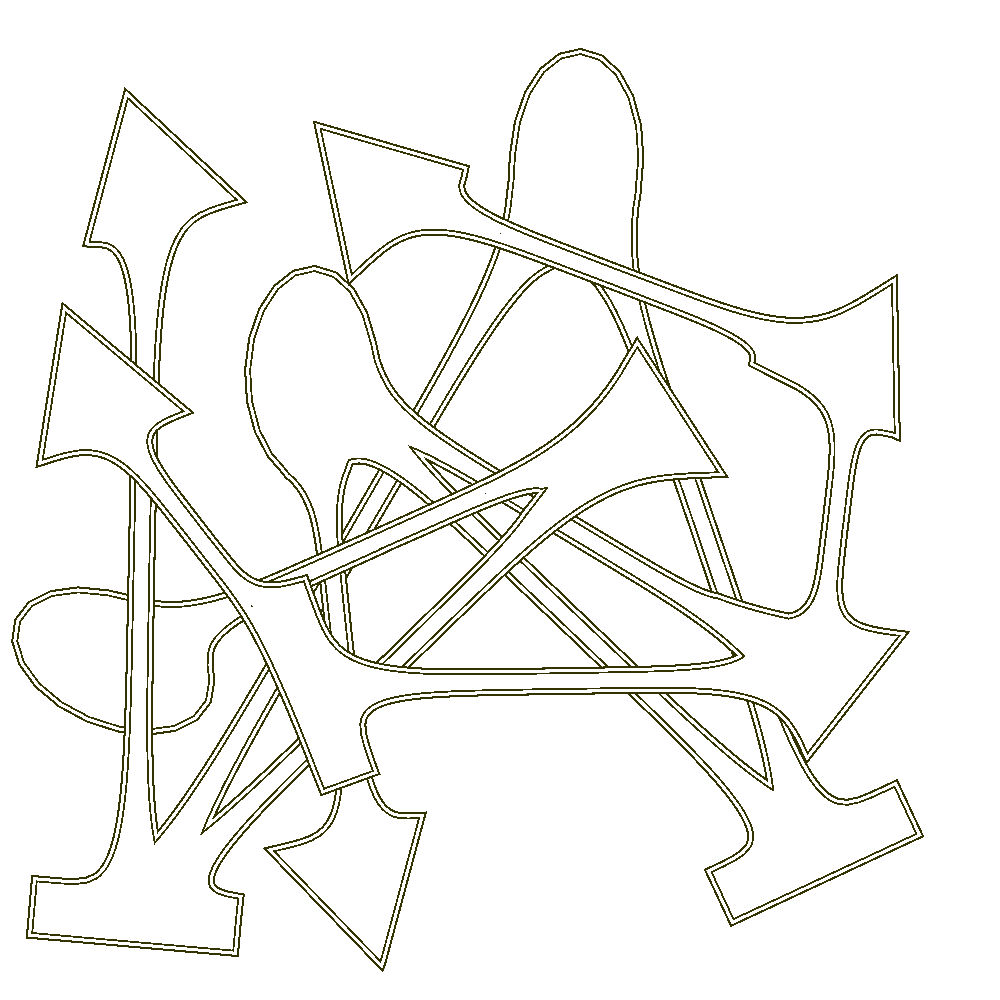
\includegraphics[width=7cm]{scene-outline.eps}
\caption{A random, badly laid out graph rendered using the general algorithm.
The image has been rendered with narrow, double lines at the edge
to show that a general 1D texture can be used at the edges without 
problems, due to the beveling and Z-buffering. Unfortunately this 
degrades the quality of the image on paper somewhat.
\label{fig-general-algorithm-example}
}
\end{figure}

\begin{figure}
\centering

\includegraphics[width=7cm]{scene-bevel.eps}
\caption{The same scene rendered using the general algorithm, with
beveling using OpenGL lighting.
\label{fig-general-algorithm-trid}
}
\end{figure}

\begin{figure}
\centering
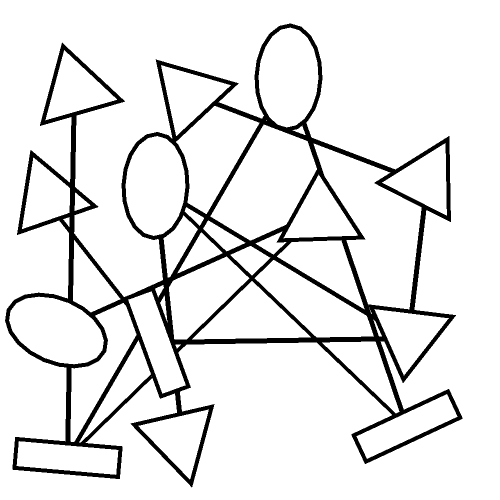
\includegraphics[width=7cm]{scene-line.eps}
\caption{The same scene rendered in the conventional way with lines. 
\label{fig-general-algorithm-conventional}
}
\end{figure}

% 
% \subsection{Obtaining Example Code}
% 
% Program code for all screenshots is available as part
% of the Gzz\cite{gzz} prototype, which is Free (libre) Software, distributed
% under the GNU LGPL. There is currently no stable, released version
% but the CVS version control system is open for anonymous access,
% and we hope to release version 0.8.0 (\emph{chartreuse}) shortly.





\end{document}

